% Results section, numbers from evaluations/ground_truth/*.json (config: configs/ground_truth.json)

\subsection{Choice of the noise scales}\label{sec:tuning}
The scales $\sigma_h,\sigma_J$ set how ``protein-like'' the sequences are. Too weak, and sequences are
almost random: our first try ($\sigma_h^{(0)}=1$, $\sigma_J^{(0)}=0.5$) gave only 18\% identity
within a clade, and correlations on contacts were barely above noise. Too strong, and the model
freezes into a few sequences and Gibbs mixes slowly. We scanned four settings and kept
$\sigma^{(0)}_h=1.5$, $\sigma^{(0)}_J=0.8$. With these, the mean site entropy is $\approx1.6$ nats
(the maximum, $\log 20$, is 3.0), identity is $\approx34\%$ within a clade and $\approx15\%$
between families (real families typically sit at 25--40\%), and the energy autocorrelation is gone
within 20 sweeps.

\subsection{The hierarchy of the models (on $J$ and $h$)}
\begin{figure}[H]
\centering
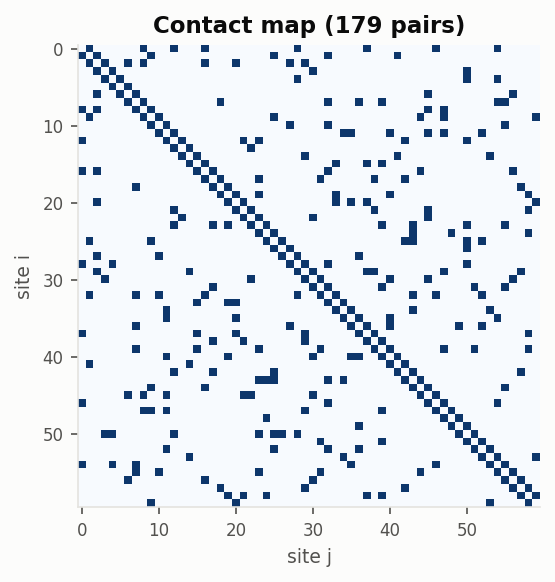
\includegraphics[width=0.3\linewidth]{ground_truth/01_hierarchy/contact_map.png}\hfill
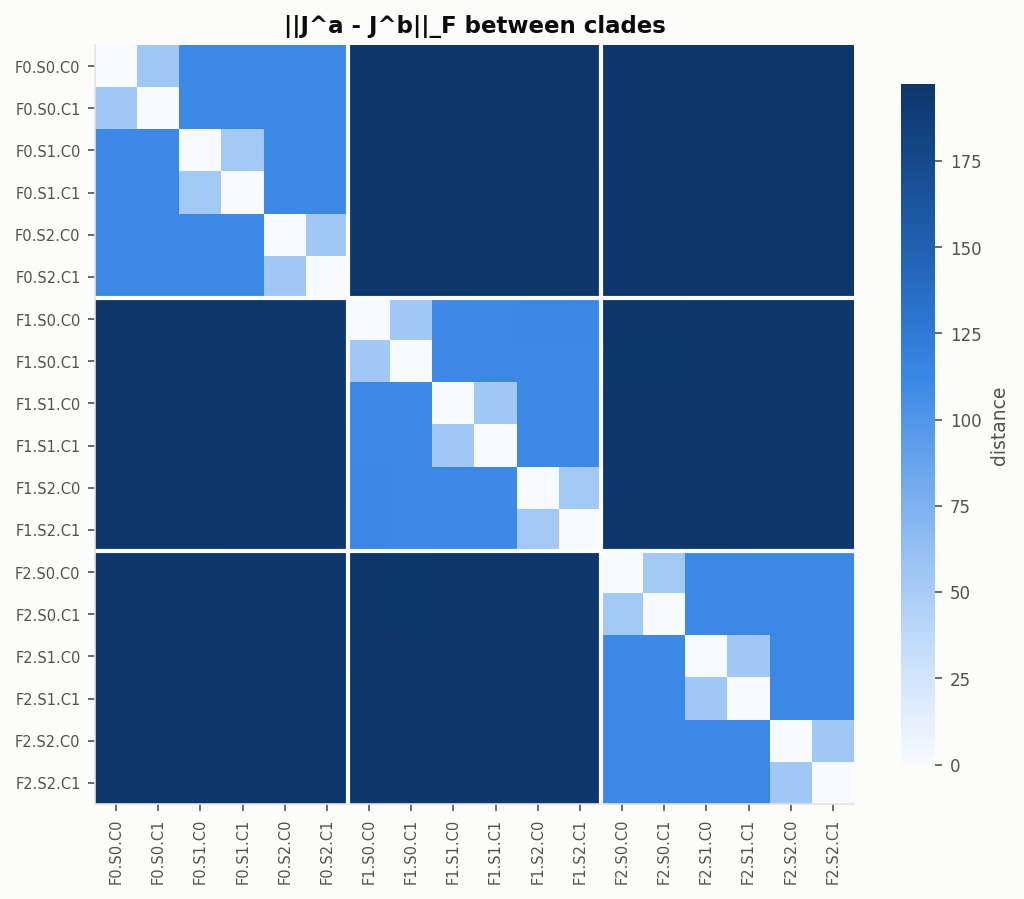
\includegraphics[width=0.66\linewidth]{ground_truth/01_hierarchy/J_distance_matrix.png}
\caption{Left: the shared contact map (59 backbone + 120 long-range pairs). Right:
$d_J=\|J^{0,a}-J^{0,b}\|_F$ between the 18 clades, ordered by family / subfamily / clade. The
nested block structure is the hierarchy.}
\label{fig:contacts}
\end{figure}

\begin{figure}[H]
\centering
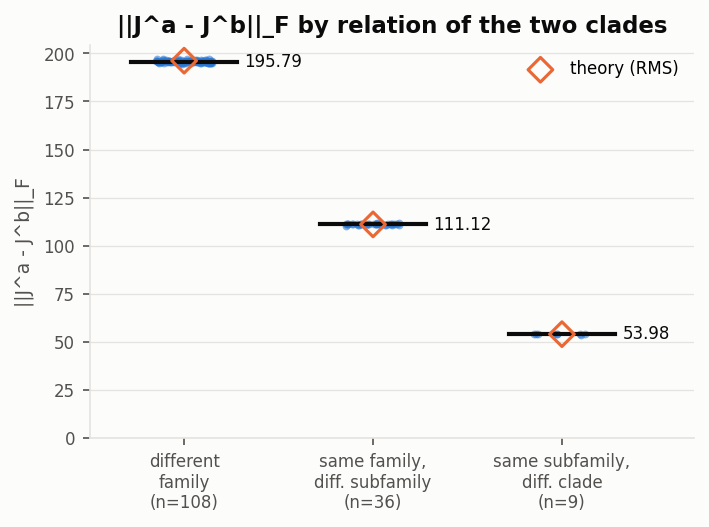
\includegraphics[width=0.49\linewidth]{ground_truth/01_hierarchy/J_distance_by_relation.png}\hfill
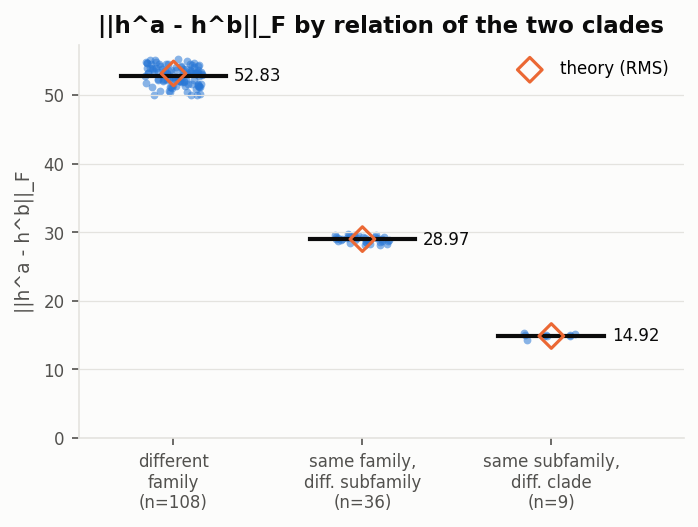
\includegraphics[width=0.49\linewidth]{ground_truth/01_hierarchy/h_distance_by_relation.png}
\caption{Distances between pairs of clades, grouped by the level of their common ancestor.
Dots are pairs, black bars their mean, orange diamonds the theoretical RMS from
\eqref{eq:dJ}--\eqref{eq:dh}.}
\label{fig:dist}
\end{figure}

\begin{center}\small
\begin{tabular}{lccccc}
\toprule
relation & pairs & $d_J$ range & $d_J$ RMS & theory \eqref{eq:dJ} & $d_h$ RMS (theory \eqref{eq:dh})\\
\midrule
different family & 108 & 194.7 -- 197.1 & 195.8 & 196.2 & 52.8 (53.2)\\
same family, diff.\ subfamily & 36 & 110.4 -- 111.7 & 111.1 & 111.0 & 29.0 (29.0)\\
same subfamily, diff.\ clade & 9 & 53.7 -- 54.2 & 54.0 & 53.9 & 14.9 (14.9)\\
\bottomrule
\end{tabular}
\end{center}
\textbf{Check passed:} the ordering is strict (the ranges do not overlap) for both $J$ and $h$, and
the measured distances agree with the closed-form prediction to within 0.5\% for $J$ and 1\% for $h$.
The models are therefore hierarchically different in exactly the designed way.

\subsection{Sampling}
18 clades $\times$ 2000 independent chains $\times$ 200 sweeps, about 33\,s per clade.
Over the last 100 sweeps, the energy autocorrelation averaged over clades is $\rho(1)=0.44$,
$\rho(5)=0.11$, $\rho(20)=-0.03$, and the mean energy drifts by less than $0.2$ (on energies of about
$-260$ to $-290$) between the third and fourth quarters of the run: the chains are at equilibrium.

\begin{figure}[H]
\centering
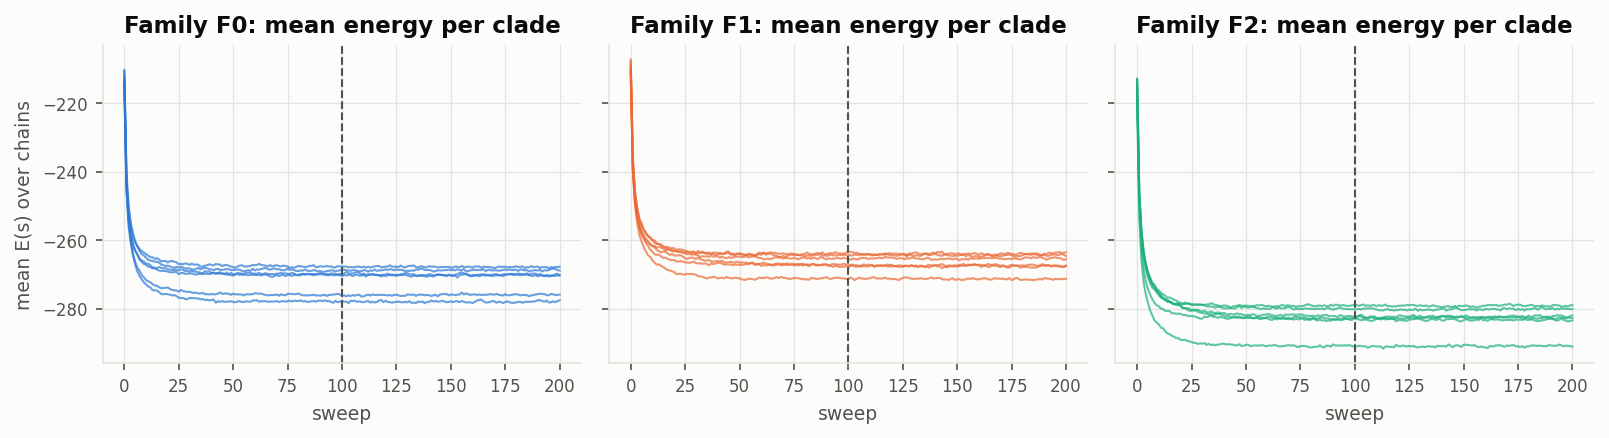
\includegraphics[width=0.95\linewidth]{ground_truth/02_sampling/energy_traces.png}
\caption{Mean energy over 2000 chains vs.\ sweep, one line per clade. The energy reaches its plateau within 20--50
sweeps; the dashed line marks the start of the window used for the diagnostics.}
\label{fig:energytraces}
\end{figure}

\subsection{PCA}
The PCA is fitted on all 36{,}000 sequences. PC1 and PC2 explain $7.2\%$ and $5.0\%$ of the variance;
the next ones about $1\text{--}2\%$ each. That low percentage is normal: the 1200-dimensional one-hot
space is dominated by site-wise noise. The two leading PCs are exactly the ``between-family''
directions (three families need two dimensions to be separated), so the three families form three
disjoint clouds (Figure~\ref{fig:pca}). Within one family (PCA fitted on that family only), the three
subfamilies separate, with some overlap. Clades, the finest level, do not separate visibly in two
dimensions. The metrics below show they are nonetheless statistically different.

\begin{figure}[H]
\centering
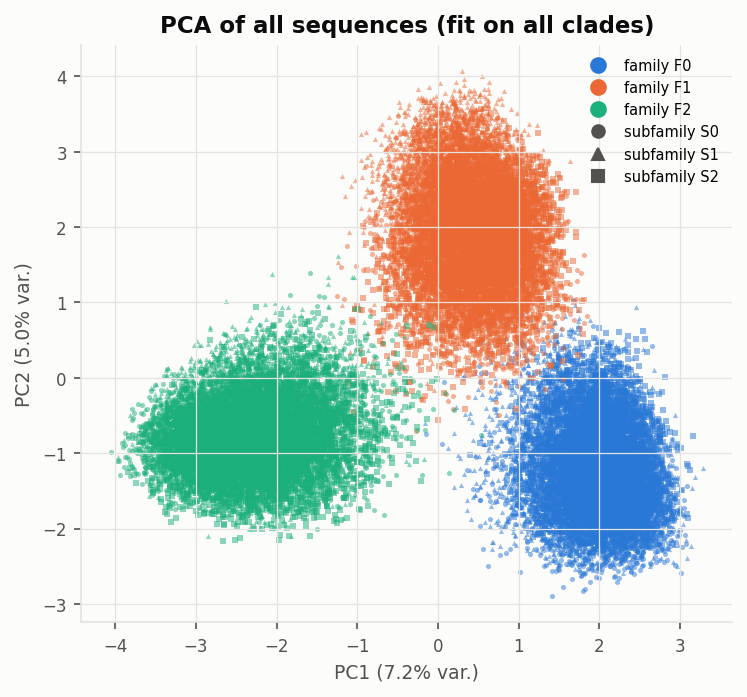
\includegraphics[width=0.55\linewidth]{ground_truth/03_analysis/pca_all_PC1_PC2.png}
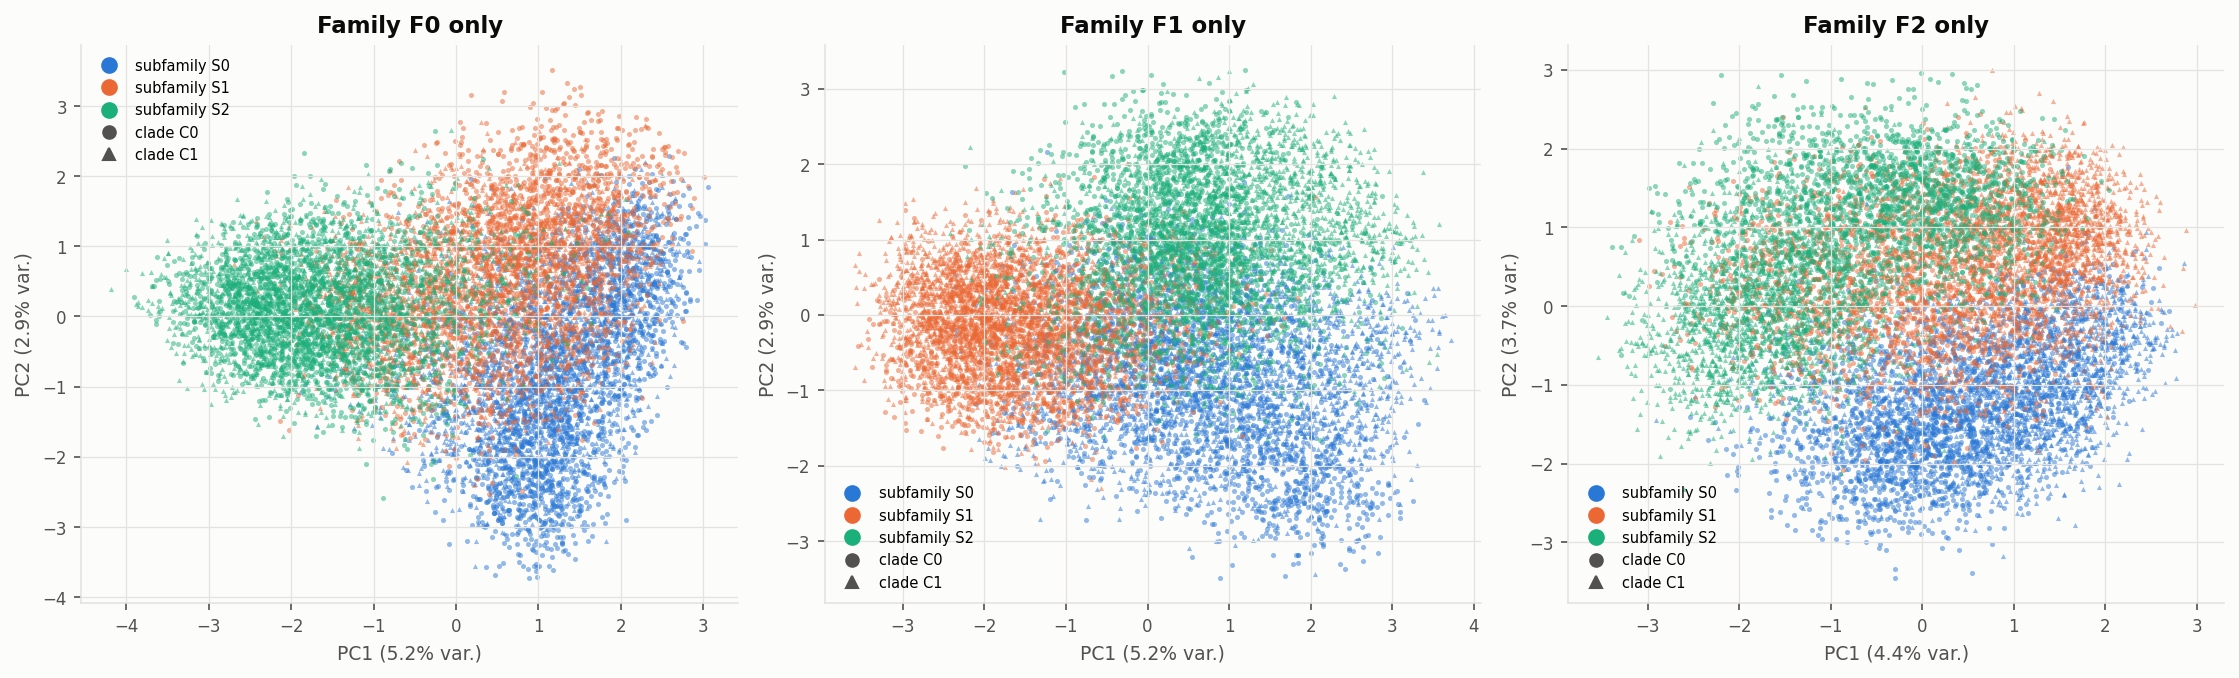
\includegraphics[width=\linewidth]{ground_truth/03_analysis/pca_within_family.png}
\caption{Top: all sequences on the reference PCA axes, colour = family, marker = subfamily. Bottom:
one PCA per family, colour = subfamily, marker = clade.}
\label{fig:pca}
\end{figure}

\subsection{Frequencies and correlations}
\begin{figure}[H]
\centering
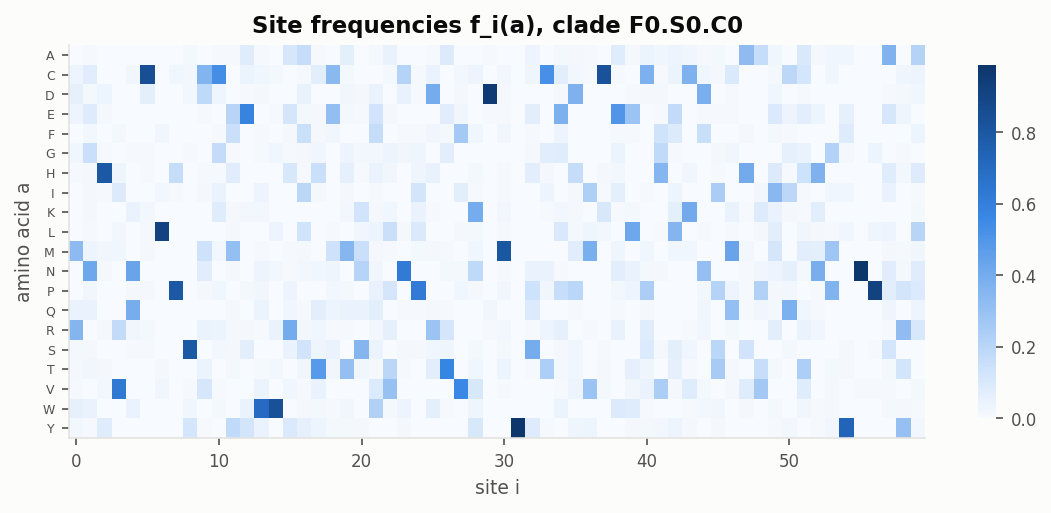
\includegraphics[width=0.52\linewidth]{ground_truth/03_analysis/site_frequencies_F0.S0.C0.png}\hfill
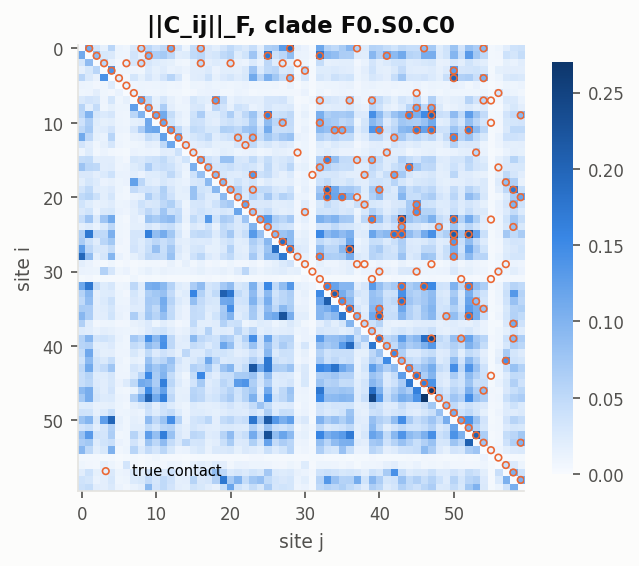
\includegraphics[width=0.44\linewidth]{ground_truth/03_analysis/correlation_strength_F0.S0.C0.png}
\caption{Clade \texttt{F0.S0.C0}. Left: $f_i(a)$; dark cells are conserved residues. Right: the
strength $\|C_{ij}\|_F$ of each pair's correlation, with true contacts circled (upper triangle).}
\label{fig:corr}
\end{figure}
The mean correlation strength is $0.100$ on contact pairs and $0.035$ on non-contacts. Contacts are
clearly enriched, but many non-contacts are correlated as well. These are the \emph{indirect}
correlations of \S\ref{sec:stats}, plus finite-sample noise. Rows that are almost blank (e.g.\ site
31) are highly conserved sites: a site that barely varies cannot co-vary with anything.

\subsection{The metric and its reference values}\label{sec:refvalues}
We compute the metric of \S\ref{sec:metric} between every pair of clades, and between two halves of
each clade (the noise floor):

\begin{center}
\begin{tabular}{lccc}
\toprule
compared sets & $r_f$ (mean) & $r_C$ (mean [min, max]) & identity\\
\midrule
same clade, two halves of 1000 (\textbf{noise floor}) & 0.998 & 0.83 [0.80, 0.88] & 0.34\\
same subfamily, different clade & 0.90 & 0.63 [0.55, 0.69] & 0.31\\
same family, different subfamily & 0.75 & 0.35 [0.25, 0.46] & 0.27\\
different family & 0.37 & 0.08 [0.04, 0.13] & 0.15\\
\bottomrule
\end{tabular}
\end{center}

\begin{figure}[H]
\centering
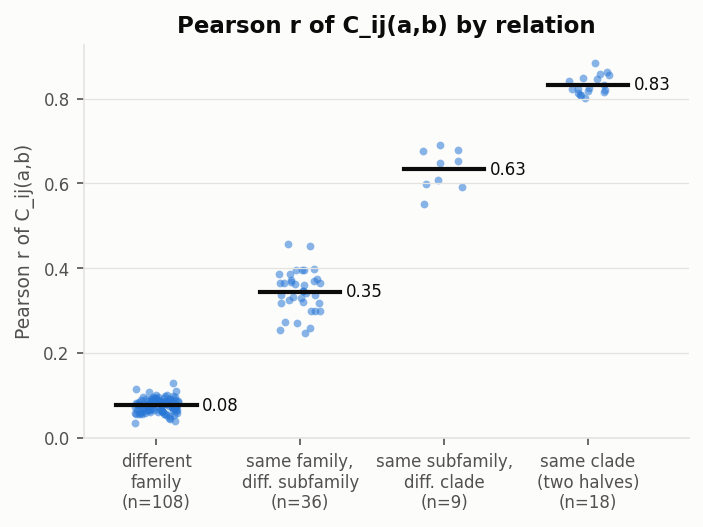
\includegraphics[width=0.49\linewidth]{ground_truth/03_analysis/pearson_C_by_relation.png}\hfill
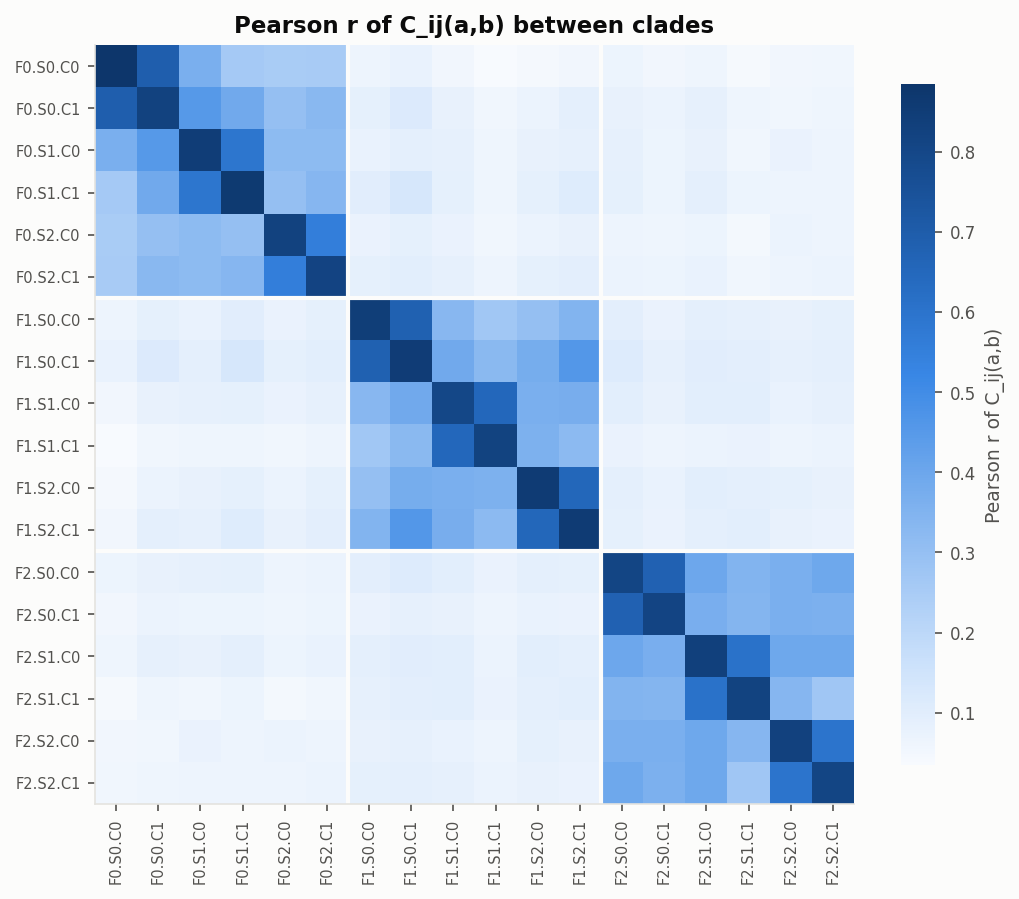
\includegraphics[width=0.49\linewidth]{ground_truth/03_analysis/pearson_C_matrix.png}
\caption{Pearson $r_C$ of the connected correlations. Left: grouped by relation. Right: all
clade pairs (the diagonal is the half-vs-half noise floor).}
\end{figure}

\begin{figure}[H]
\centering
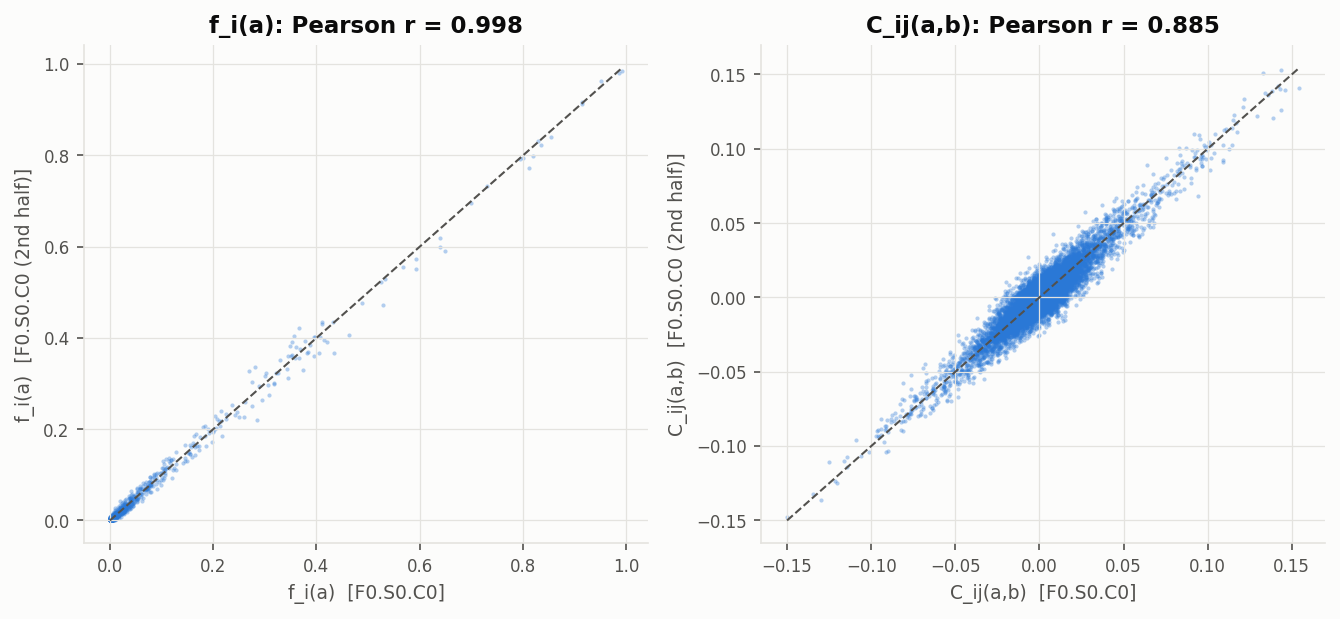
\includegraphics[width=0.49\linewidth]{ground_truth/03_analysis/compare_same_clade_halves.png}\hfill
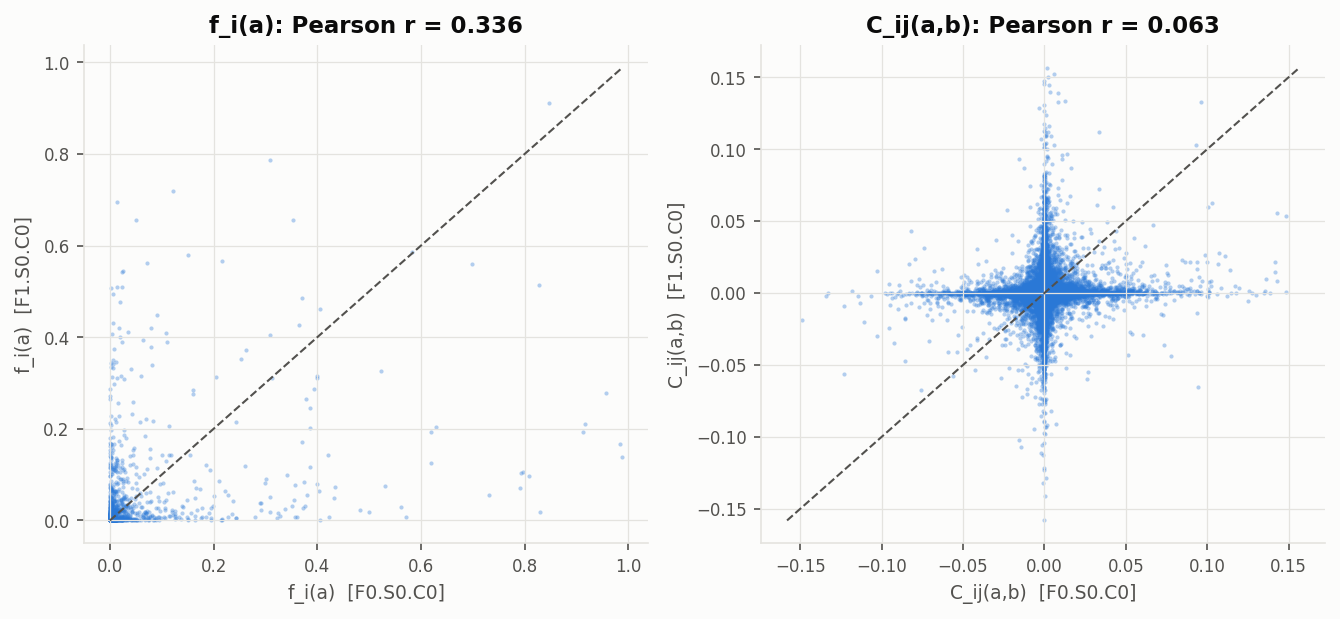
\includegraphics[width=0.49\linewidth]{ground_truth/03_analysis/compare_other_family.png}
\caption{Scatter of statistics. Left: two halves of the same clade (the best achievable). Right:
the same clade vs.\ a clade of another family (what a generator that got the family wrong would
score).}
\end{figure}

\begin{keybox}{How to read a future generative model's score}
For a model asked to generate clade $X$, compute $r_C$ against the held-out ground-truth sequences of
$X$ at matching sample size. Values near $0.83$ mean it reproduces the clade as well as fresh
ground-truth samples would. About $0.63$ means it only captured the subfamily, about $0.35$ only the
family, and below $0.1$ it is not even the right family. Note that $r_C$ depends on sample size
(noise), so compare at the same $M$.
\end{keybox}
